\begin{figure}[htbp]
    \centering
    % First TikZ picture
    \begin{subfigure}[b]{0.45\textwidth}
        \centering
        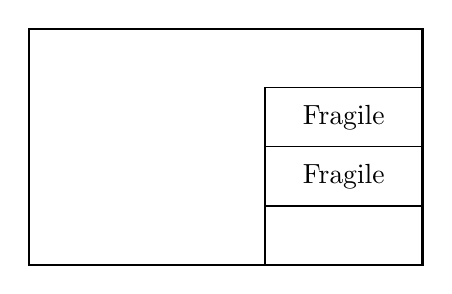
\begin{tikzpicture}
            % Draw the container
            \draw[thick] (0,0) rectangle (5,3);

            % Draw the three items inside
            \draw[] (3,0) rectangle (5,0.75);
            \node at (4, 0.5) {};

            \draw[] (3,0.75) rectangle (5,1.5);
            \node at (4, 1.125) {Fragile};

            \draw[] (3,1.5) rectangle (5, 2.25);
            \node at (4, 1.875) {Fragile};

        \end{tikzpicture}
        \caption{Feasible stacking of the items}
    \end{subfigure}
    \hfill
    % Second TikZ picture
    \begin{subfigure}[b]{0.45\textwidth}
        \centering
        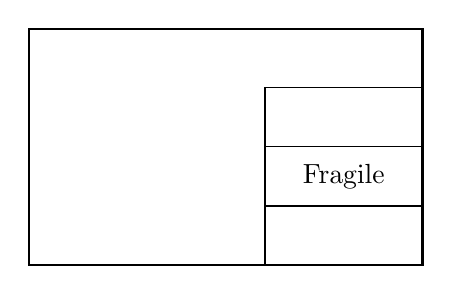
\begin{tikzpicture}
            \draw[thick] (0,0) rectangle (5,3);

            % Draw the three items inside
            \draw[] (3,0) rectangle (5,0.75);
            \node at (4, 0.5) {};

            \draw[] (3,0.75) rectangle (5,1.5);
            \node at (4, 1.125) {Fragile};

            \draw[] (3,1.5) rectangle (5, 2.25);
            \node at (4, 1.875) {};
        \end{tikzpicture}
        \caption{Non-feasible stacking of the items}
    \end{subfigure}
    \caption{Comparison fragile stacking}
    \label{fig:stacking_comparison}
\end{figure}
